\documentclass[tikz,border=2pt]{standalone}
\usepackage{amsmath,amssymb}
\usepackage{tikz}
\usetikzlibrary{arrows.meta}

\begin{document}
% Orthogonal vectors meet at a right angle; algebraically their dot product vanishes.
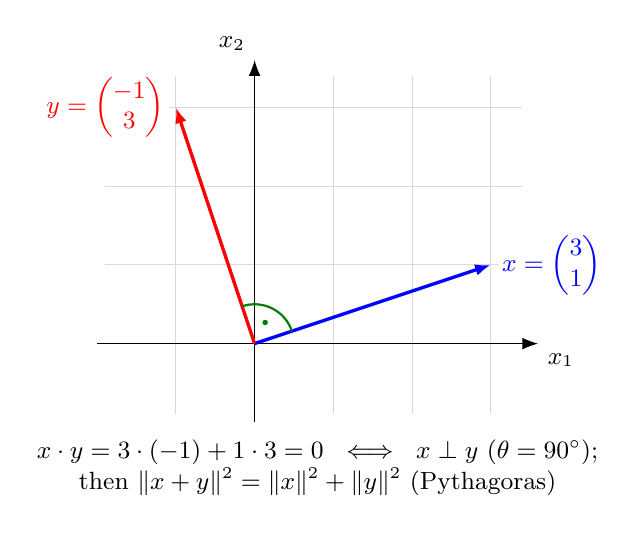
\begin{tikzpicture}[every node/.style={font=\small}, >={Latex[length=2mm]}]
	\draw[gray!30, step=1] (-1.9,-0.9) grid (3.4,3.4);
	\draw[->] (-2,0) -- (3.6,0) node[below right] {$x_1$};
	\draw[->] (0,-1) -- (0,3.6) node[above left] {$x_2$};
	\draw[->, blue, very thick] (0,0) -- (3,1) node[right, fill=white, inner sep=1.5pt, xshift=2pt] {$x=\begin{pmatrix}3\\1\end{pmatrix}$};
	\draw[->, red, very thick] (0,0) -- (-1,3) node[left, fill=white, inner sep=1.5pt, xshift=-2pt] {$y=\begin{pmatrix}-1\\3\end{pmatrix}$};
	\draw[green!50!black, thick] (18.4:0.5) arc (18.4:108.4:0.5);
	\fill[green!50!black] (63.4:0.3) circle (1pt);
	\node[anchor=north, align=center] at (0.8,-1.1) {$x\cdot y=3\cdot(-1)+1\cdot3=0\ \iff\ x\perp y$ ($\theta=90^\circ$);\\ then $\|x+y\|^2=\|x\|^2+\|y\|^2$ (Pythagoras)};
\end{tikzpicture}
\end{document}
